% This thesis template is based on the personal template of Felix Moebius. Thanks, Felix!
% It has been extended and modified by Tobias Pfandzelter at the Scalable Software Systems group of TU Berlin.
% It is licensed under the terms of the MIT license, meaning you are free to use it however you see fit but we accept no liability.
% Good luck writing your thesis!

\documentclass[a4paper, 11pt]{article}

\usepackage[utf8]{inputenc}
\usepackage[T1]{fontenc}
\usepackage{fix-cm}

\usepackage[a4paper, margin=3cm]{geometry}
\usepackage[titletoc, title]{appendix}

\usepackage{color}
\usepackage{booktabs}
\usepackage[all]{nowidow}
\usepackage[dvipsnames]{xcolor}
\usepackage[hidelinks]{hyperref}
\usepackage{acronym}
\usepackage{graphicx}
\usepackage{adjustbox}
\usepackage{url}
\urlstyle{same} % changes the font of URLs to the same as the rest of the text
\usepackage{titlesec}
\usepackage{csquotes}

\usepackage{transparent}
\usepackage{eso-pic}
\usepackage[section]{placeins}
\usepackage{setspace}
\usepackage{parskip}
\usepackage{subcaption}

\renewcommand\thefigure{%
\thesection.\arabic{figure}}
\renewcommand\thesubfigure{%
\thesection.\arabic{figure}.\arabic{subfigure}}
\renewcommand\thetable{%
\thesection.\arabic{table}}

\usepackage[main=english, ngerman]{babel}

% we use the cleveref package to refer to figures, sections, etc.
% instead of "Figure~\ref{fig:example}", write only "\cref{fig:example}" and the word "Figure" (or table, etc) will be inserted normally
\usepackage[noabbrev,capitalise]{cleveref}
\usepackage[final,nopatch=footnote]{microtype}

\usepackage[
    maxbibnames=99,
    % style=alphabetic,
    style=numeric,
    url=false,
    backend=biber,
    sortcites=true,
]{biblatex}
\addbibresource{refs.bib}
\DeclareFieldFormat[online]{urldate}{Last accessed: #1}
\DeclareFieldFormat{eprint}{arXiv: \href{https://arxiv.org/abs/#1}{#1}}
\DeclareFieldFormat[report]{title}{``#1''}
\graphicspath{ {./fig/} }

\newcommand{\projectTitle}{Practical FaaS Performance Variability Implications in the Serverless Image Optimization Scenario}
\newcommand{\thesisType}{Master's Thesis}
\newcommand{\authors}{Piotr Witkowski}
\newcommand{\matrikel}{414360}
\newcommand{\authorEmail}{\href{mailto:witkowski@campus.tu-berlin.de}{witkowski@campus.tu-berlin.de}}
\newcommand{\examinera}{Prof.~Dr.-Ing.~David Bermbach}
\newcommand{\examinerb}{Prof.~Dr.~habil.~Odej Kao}
\newcommand{\supervisor}{Trever Schirmer}

\newcommand{\projectYear}{2025}
\newcommand{\facultyName}{Fakultät Elektrotechnik und Informatik}
\newcommand{\departmentName}{Fachgebiet Scalable Software Systems}

\begin{document}
\input{front.tex}

\newpage

\section*{Abstract}
The research investigates performance variability in Function-as-a-Service (FaaS) platforms when applied to serverless image optimization workloads. Through a comprehensive two-month benchmark comparing AWS Lambda and Google Cloud Run functions, the study quantifies various aspects of serverless performance including cold starts, environment reuse patterns, hardware allocation inconsistencies, and temporal performance variations. The benchmark utilized a systematic approach with 108 distinct function variants processing different image types across multiple performance configurations. Results reveal significant differences between platforms: AWS Lambda experienced cold starts 48 times more frequently than Google Cloud Run, but consistently delivered faster absolute processing times. Google Cloud environments demonstrated remarkable longevity, sometimes persisting for over 20 days and handling thousands of requests, while Lambda environments typically lasted under 2 hours. Both platforms exhibited daily and weekly performance fluctuations of 1-2\%, with higher variability observed for compute-intensive formats. The findings provide valuable insights for developers implementing serverless image optimization solutions, highlighting the trade-offs between cold start frequency, processing speed, environment stability, and infrastructure reliability across platforms.

% GERMAN
\clearpage
\begin{otherlanguage}{ngerman}
\section*{Kurzfassung}
Die Forschung untersucht die Leistungsvariabilität in Function-as-a-Service Plattformen bei der Anwendung auf serverlose Bildoptimierungs-Workloads. Die Studie vergleicht in einem umfassenden zweimonatigen Benchmark AWS Lambda- und Google Cloud Run-Funktionen und quantifiziert verschiedene Aspekte der serverlosen Leistung, darunter Kaltstarts, Muster der Umgebungswiederverwendung, Inkonsistenzen bei der Hardwarezuweisung und zeitliche Leistungsvariabilität. Für den Benchmark wurde ein systematischer Ansatz mit mehr als 100 verschiedenen Funktionsvarianten verwendet, die unterschiedliche Bildtypen in verschiedenen Leistungskonfigurationen verarbeiten. Die Ergebnisse zeigen signifikante Unterschiede zwischen den Plattformen: AWS Lambda erlebte 48 Mal häufiger Kaltstarts als Google Cloud Run, lieferte aber durchweg schnellere absolute Verarbeitungszeiten. Google Cloud-Umgebungen wiesen eine bemerkenswerte Langlebigkeit auf, die manchmal über 20 Tage anhielt und Tausende von Anforderungen verarbeitete, während Lambda-Umgebungen in der Regel weniger als 2 Stunden dauerten. Beide Plattformen wiesen tägliche und wöchentliche Leistungsschwankungen von 1 bis 2 \% auf, wobei bei rechenintensiven Formaten eine höhere Variabilität beobachtet wurde. Die Ergebnisse liefern wertvolle Erkenntnisse für Entwickler, die serverlose Bildoptimierungslösungen implementieren, und zeigen die Kompromisse zwischen Kaltstarthäufigkeit, Verarbeitungsgeschwindigkeit, Stabilität der Umgebung und Zuverlässigkeit der Infrastruktur auf verschiedenen Plattformen auf.
\end{otherlanguage}

\clearpage

\enlargethispage{2\baselineskip}
\tableofcontents

\section{Introduction}
\label{cha:introduction}

The digital revolution has fundamentally transformed the way we create, consume, and interact with visual information.
Images are no longer only physical items around us, they are inherent components of our online experience, shaping perceptions and influencing decisions.
As the Internet continues to evolve, so too grows the demand for rich and engaging visual content.
This demand, however, comes at a cost. Images, while visually appealing, are significantly impacting website performance, not only by generating the highest number of requests, but also by consuming the most bytes during page load of an average site.
Existing studies have shown a strong correlation between page load times and user engagement, conversion rates, and even search engine rankings.
Minimizing image size is therefore fundamental for efficient bandwidth use and plays a crucial role in optimizing website performance.

Image optimization practices for the web have evolved over time, following developments of the state-of-the-art image formats and codecs.
These solutions perform operations such as image resizing and format conversion, and may allow for storing optimized versions of original files for future use.
While the optimization itself is a relatively specialized task, its deployment models follow familiar and established patterns in the general software industry: we can find them in software-as-a-service offerings, integrated into web hosting and content delivery platforms, but also as open-source solutions for self-hosting.

This last option, leveraging open-source image processing libraries, presents a compelling opportunity for our research.
Unlike proprietary solutions, open-source projects offer the flexibility to be deployed across a variety of environments, granting builders granular control over the optimization process.
This allows not only to measure influence of different libraries and optimization parameters, but also – and crucially for this thesis – enables realistic benchmarking of the underlying platforms on which these operations are performed.
By employing these workloads, our research aims to accurately measure cloud service performance under the realistic conditions of real-world image optimization scenarios.

Given the event-driven nature of the optimization workload in response to requests for images, serverless cloud compute emerges as a well-suited deployment option for these systems.
However, the varying demands for image processing, including different image sizes and diverse range of image formats present on the web, raise questions about the suitability and performance consistency of these platforms for the use-case.
Furthermore, the emergence of function as a service (FaaS) platforms introduces a new dimension to cloud-based, self-hosted image optimization.
FaaS offers a compelling execution environment for image processing tasks thanks to its on-demand scalability and event-driven nature.
However, the performance variability inherent in FaaS platforms, attributed to diverse factors, may impact efficiency of the process and applicability of the environment for the use case.


\subsection{Objectives of the Thesis}
This thesis aims to investigate whether FaaS performance variability has measurable and meaningful influence for image optimization workloads.
We will define set of representative metrics related to image optimization, reflecting realistic web usage.
We will design and implement the optimization workflows for selected serverless environments.
We will design and implement scheduling mechanism allowing us to simulate requests for optimized images.
We will collect performance metrics across all parameters, apply statistical methods for result comparisons, and visualize the results.
We will investigate if more intensive optimization can be cost-efficient, considering optimization result caching, and content reuse for multiple viewers.
We will provide recommendations that are within the scope of the benchmark, and answer the primary research question in the context of the scenario. 


\subsection{Structure}
Provide a roadmap for the reader, outlining the organization of the thesis and briefly summarizing the content of each chapter.

\clearpage
\section{Background}
\label{cha:background}

This chapter provides readers with foundations for understanding the challenges and opportunities of serverless image processing. We begin by revisiting fundamental principles of imaging and photography. Subsequently, we describe core digital imaging concepts, emphasizing aspects relevant to web performance. We then examine the characteristics of serverless cloud computing, focusing on factors contributing to performance variability. Finally, we explore image optimization for the web, reviewing established techniques and the landscape of cloud-based solutions.

\subsection{Imaging and Photography}
\label{sec:imaging-and-photography}
% Discuss the transition from analog to digital photography.
% "The best camera is the one that's with you" - Chase Jarvis

\textit{Imaging} is a broad term describing any process that helps us in visualizing and understanding physical objects, abstract concepts, or even sets of data. While this may be a purely philosophical activity, for the purpose of this thesis, we will define imaging as creating a visual representation - \textit{an image} - of physical objects and scenes. Humans are able to perceive and interpret these images thanks to our visual system, that has evolved over millions of years. Developed from the simple light-sensitive cells of early organisms to the sophisticated eyes of modern humans, this system is providing us with the ability to see color, depth, or movement.

Over centuries, scholars and artists showed great interest in this process of creating visual representations to understand our own senses, as well as to be able to depict the world around us more accurately. The natural phenomenon of light passing through a small aperture, called camera obscura, helped us understand fundamental principles of optics and image formation, and according to some, greatly contributed to realism of European art during Middle Ages. We've been refining tools and techniques to enhance our vision, and improve everyday life. Devices like telescopes and microscopes allowed us to observe objects at different scales, unveiling worlds that would otherwise remain invisible to the naked eye. Eyeglasses and contact lenses correct refractive errors, demonstrating that our visual experiences can not only be externally altered, but also subjectively improved, for millions of people.

Photography emerged in the 19th century as a groundbreaking invention, offering a novel approach to image creation. Unlike paintings or drawings, which rely on an artist's interpretation, photography directly captures and permanently records the physical world using light-sensitive materials. Early photographic methods required long exposure times, often making it possible to photograph only still objects and posed portraits. The daguerreotype, which used a silver-coated copper plate, was one of the first widely adopted photographic processes. Later, more versatile film technologies significantly reduced exposure times and made photography more accessible to the wider public. This ability to easily and accurately record the physical world had significant consequences. Newspapers, now able to include actual photographs, found a powerful new way to share news and social commentary through photojournalism. On a personal level, photography allowed people to preserve their own histories through portraits and the documentation of special occasions.

Since the beginning of the 21st century, digital photography has become the dominant form of capturing and sharing images. Initially limited to standalone devices, digital cameras are now integrated into smartphones and personal computers. Electronic sensors capture and convert light into digital data, facilitating easy manipulation and image sharing, including over the Internet. This digital nature has led to the popularity of standardized formats, ensuring compatibility across diverse platforms.

However, the ease of image creation and sharing, coupled with the vast amount of image data generated daily, may present unexpected challenges for storage and transmission. In 2024, an estimated 6 billion photos are taken daily, with 14 billion images shared on social media platforms. Especially in the context of thesis, the resulting volume of image data necessitates efficient delivery. Fortunately, optimization methods exist, relying on core concepts of image representation, encoding, and compression, to ensure efficient delivery across networks. We will explore these in the subsequent sections.
% https://photutorial.com/photos-statistics/
% https://www.statista.com/chart/10913/number-of-photos-taken-worldwide/

% https://www.statista.com/chart/5782/digital-camera-shipments/
% https://www.statista.com/chart/15524/worldwide-camera-shipments/

\subsubsection{Digital imaging and image processing}
% Trace the historical development of digital imaging, emphasizing the role of computers in its evolution.

\subsubsection{Raster and vector graphics}
% Explain the distinction between raster and vector graphics.
% Mention strengths, weaknesses, and common use cases.
% Discuss the concept of image size and its relationship to representation quality in both raster and vector formats.

\subsubsection{Image data compression}
% Describe their differences, strengths, weaknesses, and common use cases.

\subsubsection{Image formats and their usage}
% Explore image formats and compression.



% \clearpage
\subsection{Cloud Computing}
\label{sec:cloud-computing}
% Provide a concise overview of cloud computing models.

\subsubsection{Cloud deployment models}
% Different deployment models, IaaS, PaaS, SaaS, and finally serverless computing.
% Mention Free tier to reference later

\subsubsection{Event-driven architectures}
% Define Serverless and Function as a Service (FaaS), its key characteristics like automatic scaling
% Advantages and disadvantages of FaaS, e.g., reduced operational overhead, cost-efficiency
% Discuss the challenges associated with FaaS, such as vendor lock-in, cold starts, and debugging complexities
% Compare and contrast popular FaaS platforms like AWS Lambda, Google Cloud Functions, and Azure Functions
% Focusing on their features relevant to image optimization (e.g., supported runtimes, storage integrations)

\subsubsection{Cloud service benchmarking}
% How can we measure performance of the cloud and services running in the cloud?
% Shared responsibility model for the cloud

\subsubsection{Performance variability of serverless platforms}
% Provide an analysis of the factors that contribute to performance variability in FaaS environments.
% Cold starts and their impact
% Resource allocation (CPU, memory)
% Network latency
% Concurrency and queuing
% Underlying infrastructure variations



% \clearpage
\subsection{Image Optimization for the Web}
% Explain why image optimization is crucial for web performance

\subsubsection{Impact of images on browsing experience}
% Impact of images on page load times, user experience, and SEO.
% Relationship between image optimization and Core Web Vitals.

\subsubsection{Bandwidth usage, visual quality, and browser support evolution}
% Image resizing, cropping and applying compression
% Progressive loading
% Responsive web design
% Evolution of browser support for responsive images on HTML and CSS
% Evolution of browser support for image formats
% https://medium.com/hceverything/applying-srcset-choosing-the-right-sizes-for-responsive-images-at-different-breakpoints-a0433450a4a3
% https://nextjs.org/docs/app/api-reference/components/image#devicesizes

\subsubsection{Optimizing latency of image delivery}
% On-demand vs pre-optimizing images
% Inlining assets
% Preloading assets
% HTTP caching and CDNs

\subsubsection{Deployment methods for cloud-based image optimization}
% Image CDNs
% Explain how FaaS can be used to create efficient and scalable image optimization workflows.
% Discuss the benefits of serverless image optimization (e.g., on-demand scaling, cost-effectiveness, automation).
% Present examples of FaaS-based image optimization tools and services.

\clearpage
\section{System Design}
\label{cha:system-design}

In this chapter, we will describe different input parameters that we have considered while designing the image optimization benchmark, and the selection process we used to choose the distinct values of these parameters. It is necessary to focus our study on specific parameters only, as there are too many parameters that can be configured while building a general-purpose serverless image optimization system. We will present different performance-related metrics we are able to collect during image optimization process in the chosen environments, and the methodology used to collect and process these metrics.

\subsection{Benchmark Design}

The benchmark is composed of two main components:
\begin{itemize}
  \item \textbf{Workload Generation Stack}, which is responsible for generating the image optimization workload and saving the results of the optimization requests in a database. 
  \item \textbf{Image Optimization Stacks}, which are provider-specific systems under test (SUTs) that are responsible for hosting and exposing image optimization serverless functions.
\end{itemize}



Both workload generation and image optimization were implemented in a serverless fashion. For simplicity, workload generator infrastructure was all deployed in one environment - in our case it was AWS, but any cloud provider (or even no cloud infrastructure) could be used, as long as it is connected to the Internet, capable of sending HTTP requests on a schedule and storing the results in a database.

\begin{figure}[htb]
  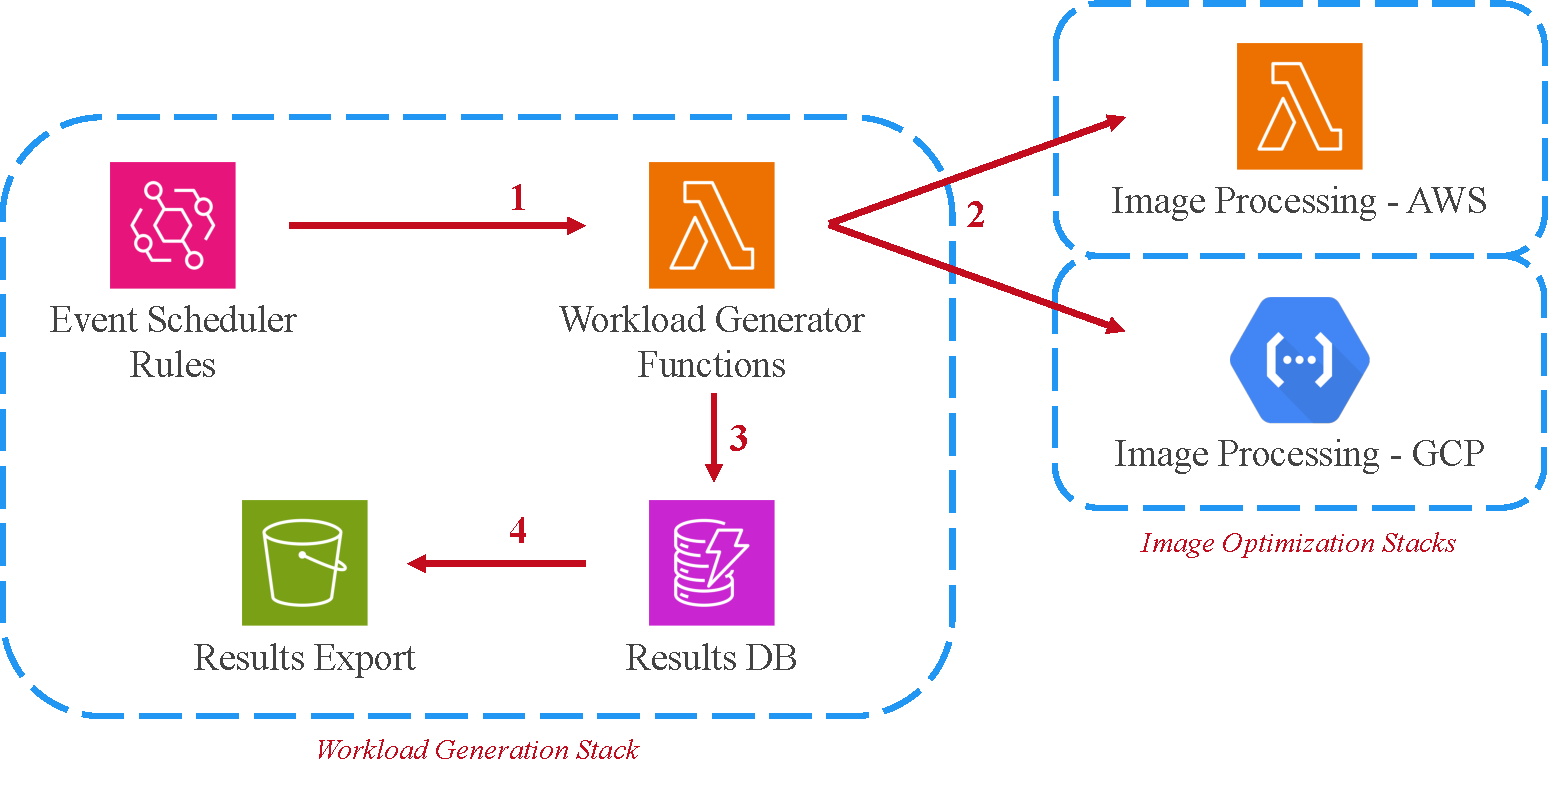
\includegraphics[width=\textwidth]{benchmark-design.pdf}
  \caption{High-level overview of the image optimization benchmark design}
  \label{fig:benchmark-design}
\end{figure}

The figure \ref{fig:benchmark-design} shows the main steps of the benchmark:
\begin{enumerate}
  \item \textbf{event scheduler} invokes the workload generator functions,
  \item \textbf{workload generators} send requests to specific image processing functions,
  \item \textbf{workload generators} save image optimization results in the database,
  \item \textbf{benchmark results} are exported as JSON to a bucket for later offline analysis.
\end{enumerate}

The image optimization stacks were deployed in two different clouds - which we call \emph{providers} - AWS and GCP. These stacks are responsible for providing HTTP endpoints and function invocation in response an incoming HTTP request. Since the optimization process is consistent\footnote{By \emph{consistent} we mean producing comparable metadata outputs for identical input and optimization parameters, sufficient for reliable benchmark comparisons. Strict bit-for-bit determinism is not implied.} enough for our purposes, functions only return the metadata of an individual optimization execution, and the output images are discarded.

The image processing function, except for the actual processing, is parsing environment variables, loading image into the function's memory, and calculating the time elapsed since the cold start, as well as the duration of the actual image processing. Figure \ref{fig:processing-code} illustrates a simplified function code, outlining the key steps from the environment setup to image processing and response generation.

\begin{figure}[ht]
  
\includegraphics[width=\textwidth]{code.pdf}
  \caption{Simplified image processing function code}
  \label{fig:processing-code}
\end{figure}

In the actual image processing functions, we do return a few more optimization properties in the response object, such as exact dimensions and formats of the input and output images, as well as their byte length. We have omitted them from the code snippet here for brevity. Please note that the image processing duration strictly relates to the actual image processing: image resizing, and optionally image reformatting. It does not include any earlier steps necessary to facilitate processing, executed either on once cold start, or on every handler function call.

Please also note that in a real-world image optimization scenario, the deployment package of a serverless function does not include any image. An additional network call, or a cloud SDK operation, is required on every function call to retrieve the original, unoptimized image from an external object storage. In our study, we are not interested in measuring performance variability of such operations, and in the interest of cloud service usage minimization we have decided to load the image into memory only once, outside the handler function definition, on a cold start.


\subsubsection{Serverless environment, image, and optimization parameter selection}

There were 5 variables for each optimization function variant, presented on figure \ref{fig:function-variants}. There were in total 108 ($2^2 \cdot 3^3 $) image optimization functions deployed. Every variant deployed as separate function to minimize interference between resources. Each function includes the request handler, as well as one unoptimized image within its deployment package (ZIP file).

To simplify operations, functions were exposed behind a single domain name per provider, and we used a predictable path-based routing to invoke a specific function. For example, \texttt{portrait-1769-webp-1920} is an ID of a function that has the portrait picture stored within, is configured to use one vCPU\footnote{AWS Lambda is using the abbreviation MB (rather than MiB) across the documentation and log messages to refer to 1,024 KB. At 1,769 MB, a Lambda function has the equivalent of one vCPU.}, is using WebP as the image output format, and 1920 is the width of the output image. The use of HTTP is crucial, as it makes the workload generation provider-agnostic.

\begin{figure}[hb]
  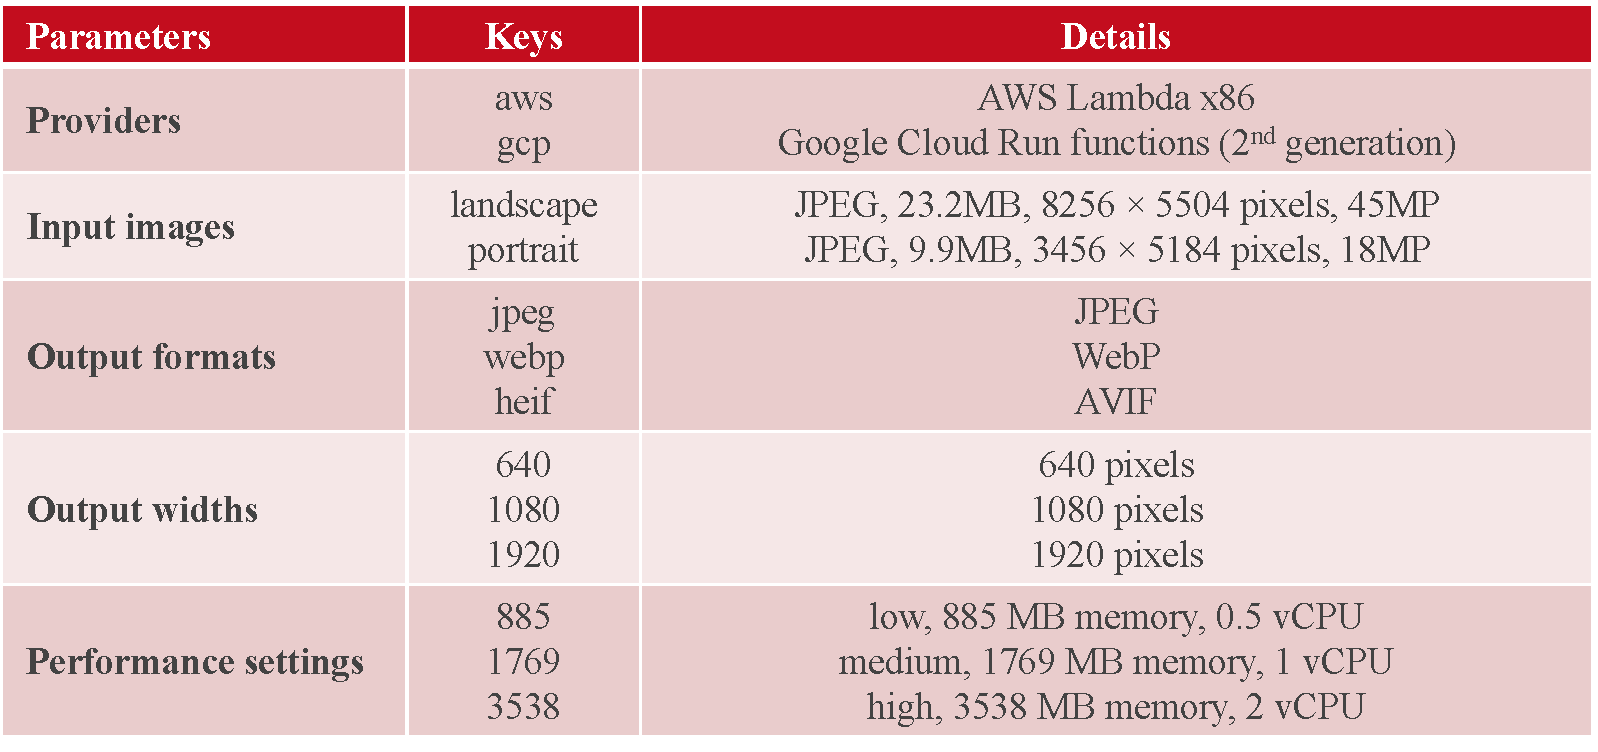
\includegraphics[width=\textwidth]{function-variants.pdf}
  \caption{All image optimization function variants deployed}
  \label{fig:function-variants}
\end{figure}

\textbf{Providers}. We have selected Lambda because of its historical significance, presence in research, as well as its market share. Cloud Run functions (2nd generation) is the new generation of the serverless platform from Google Cloud that includes improved concurrency management, and granular memory and compute configuration. We have selected this platform, as it is still relatively new (2022) offering on the Google Cloud Platform, and many studies only researched its older version.

\textbf{Input images}. To simplify function code and allow for just one optimization run per function invocation, we opted for large input images. Specifically, we selected two high-resolution images produced using DSLR cameras, one in each orientation. For this purpose, in September 2024, we visited an online stock image portal to find popular stock image categories\footnote{\url{https://pexels.com/popular-searches}}. From these popular categories, two prominent ones, namely \emph{Travel} and \emph{Summer}, were chosen, and one image from each was downloaded. Only two images were selected, because our research was primarily driven by the parametrization of the optimization process, not influence of different images on the performance variability.

\textbf{Output formats}. Three output formats were selected: JPEG (implies no reformatting), WebP, and AVIF. The latter two represent advancements in compression and browser support over the last decade. We considered, but eventually did not select JPEG XL due to its limited browser support and custom requirements around for the optimization tooling setup explained in the following section.

\textbf{Output widths}. Three widths that were chosen, 640, 1080, 1920 pixels, aim to represent different screen widths of mobile, tablet and desktop devices. Popular image optimization solutions, such as , Next.js\footnote{\url{https://nextjs.org/docs/pages/api-reference/components/image\#devicesizes}}), we typically see more granular widths used, with smaller relative differences between each next value. 

\textbf{Performance settings}.

most selecting the most popular photo category, and selecting one of the images 




For the image optimization stacks, nearby geographical regions were selected, North Virginia \texttt{(us-east-1)}, and South Carolina
\texttt{(us-east1)} for AWS and GCP, respectively. North Virginia region is the oldest AWS region, and was selected for its comparability with existing literature, such as \cite{ginzburg2020serverless}. This also guided the region choice for the GCP environment. We have not decided to parametrize the region. 

AWS Lambda allocates compute power proportionally to the amount of memory configured\footnote{\url{https://docs.aws.amazon.com/lambda/latest/dg/configuration-memory.html}}. This offers less flexibility than Google Cloud Run, where memory and compute can be configured independently\footnote{\url{https://cloud.google.com/run/docs/configuring/services/cpu\#cpu-memory}}. 



% What is exposed by serverless platforms?
% Differences in performance variability between AWS Lambda and GCP Cloud Run Functions

% Trever: What are we trying to find and ways to find it
% Why we did it 

% https://arxiv.org/pdf/2008.11110



% \subsubsection{Output formats and image widths}
% What is the influence of the output format and size on the execution time?
% AVIF / JPEG / WebP
% \subsubsection{Available CPU / memory}
% 0.5 / 1 / 2 CPUs 
% \subsubsection{Cold starts}
% Are warm functions faster/slower or the same?

% Grain of salt anti-pattern: Richards, Mark. Microservices AntiPatterns and Pitfalls. O'Reilly.


% How is this benchmark different from purely synthetic (CPU/IO-bound) perf benchmarking?
% Because of the client-oriented characteristic of the process, a real-world image optimization workloads are using user-provided parameters, such as image formats and screen width to create an appropriate, optimized image asset supported by the client.

% Clouds and region selection
% Platforms
% Runtime
% Why Node: https://ieeexplore.ieee.org/stamp/stamp.jsp?tp=&arnumber=8529465
% CPU/Memory

% Review of popular image manipulation libraries
% Why sharp/libvips
% How sharp can be configured



\subsubsection{Image manipulation library}

% What is a typical image?
% Input formats and widths
% Output formats and widths

% https://github.com/libvips/libvips/wiki/Speed-and-memory-use




\subsection{Workload Generation and Benchmark Execution}
% We will execute every function every 5 minutes
% Will hour of day or day of week influence execution duration
% How to replicate infrastructure to run the benchmark

\subsubsection{Serverless benchmark deployment}
% Compare Cloud APIs vs IaC deployments quickly

\subsubsection{Scheduling workload executions}
% Cloud-native event scheduler 

\subsubsection{Results collection and data analysis}
% Cloud-native NoSQL database was used

\clearpage
\section{Results}
\label{cha:results}

This chapter presents the results from our two-month-long benchmark of image optimization, focusing on performance metrics collected across two serverless platforms, and 54 image optimization configurations per platform. Instead of optimized images, the image optimization functions described in Section \ref{sec:results-collection-data-analysis} return a handful of characteristics, such as the cold start flag, image processing duration, and optimization invocation time. The measurements cover a period of 62 days between December 2024 and February 2025.

% ------------------------------------------------------------

% MISSED EXECUTIONS

% ------------------------------------------------------------
\subsection{Missed Executions}
Missed execution is a situation when we expect a response from the image optimization function and a corresponding record in the database, but the number of recorded observations is smaller than expected. The benchmark does not explicitly record such situation in any way, however, any error occurrences can be reasoned about by the observation of a lower than expected number of data points for a given time frame and a set of optimization parameters. For example, when surveying the results for specific function variant over a duration of one hour, 12 data points can be expected. A lower number of measurements is a very strong indicator\footnote{Due to the distributed nature of the scheduler service, there can be a delay of several seconds between the time the scheduled rule is triggered and the time the target service runs the target resource.} of missed executions of that specific functions in the selected period of time. The benchmark does not additionally track the effectiveness of the rule scheduler itself.

From exactly $1928448$ scheduled executions in total:
\begin{itemize}
  \item workload generator collected responses from $1924484$ ($99.79\%$) executions,
  \item workload generator missed responses from $3964$ ($0.21\%$) executions,
  \item $63.94$ data points were missed on an average day. 
\end{itemize}

From $964224$ scheduled executions per provider,
\begin{itemize}
  \item benchmark collected 961113 ($99.68\%$) and missed 3111 ($0.32\%$) executions from AWS,
  \item benchmark collected 963371 ($99.91\%$) and missed 853 ($0.09\%$) executions from GCP,
  \item AWS failed to deliver responses $3.65$x times more often than GCP.
\end{itemize}

\begin{figure}[ht!b]
  \centering
  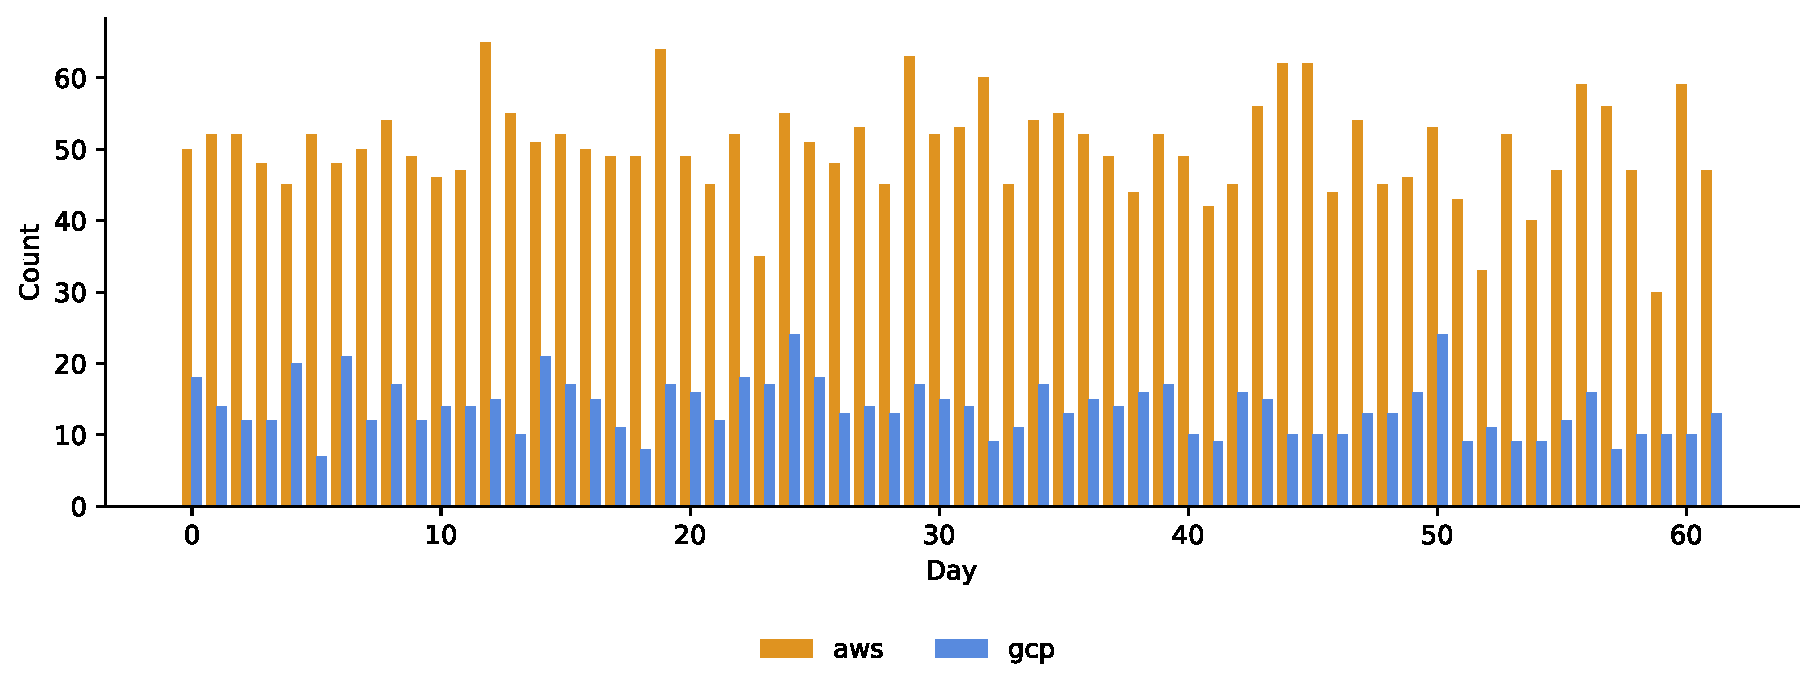
\includegraphics[width=\textwidth]{missed-executions.pdf}
  \caption{Missed executions by provider.}
  \label{fig:missed-executions-per-provider}
\end{figure}

% ------------------------------------------------------------

% COLD STARTS

% ------------------------------------------------------------
\subsection{Cold Starts}
Cold start latency is not specifically recorded as part of this benchmark. In the serverless image optimization scenario, we exclusively focus on the image optimization latency. Nevertheless, the benchmark is collecting data about an \emph{occurrence} of the cold start. This value could be inferred from the \emph{handlerCount} metric, but the optimization functions are also setting an additional property called \emph{coldStart} for convenience.

From exactly 1924484 collected responses in total:
\begin{itemize}
  \item workload generator recorded $1878363$ ($97.60\%$) warm starts,
  \item workload generator recorded $46121$ ($2.40\%$) cold starts.
\end{itemize}

From $961113$ and $963371$ of collected data points from AWS and GCP respectively,
\begin{itemize}
  \item benchmark recorded $915965$ ($95.30\%$) warm and $45148$ ($4.70\%$) cold starts on AWS,
  \item benchmark recorded $962398$ ($99.90\%$) warm and $973$ ($0.10\%$) cold starts on GCP,
  \item it was $48.18$ times more likely to observe a cold start on AWS than on GCP.  
\end{itemize}

\begin{figure}[!htbp]
  \centering
  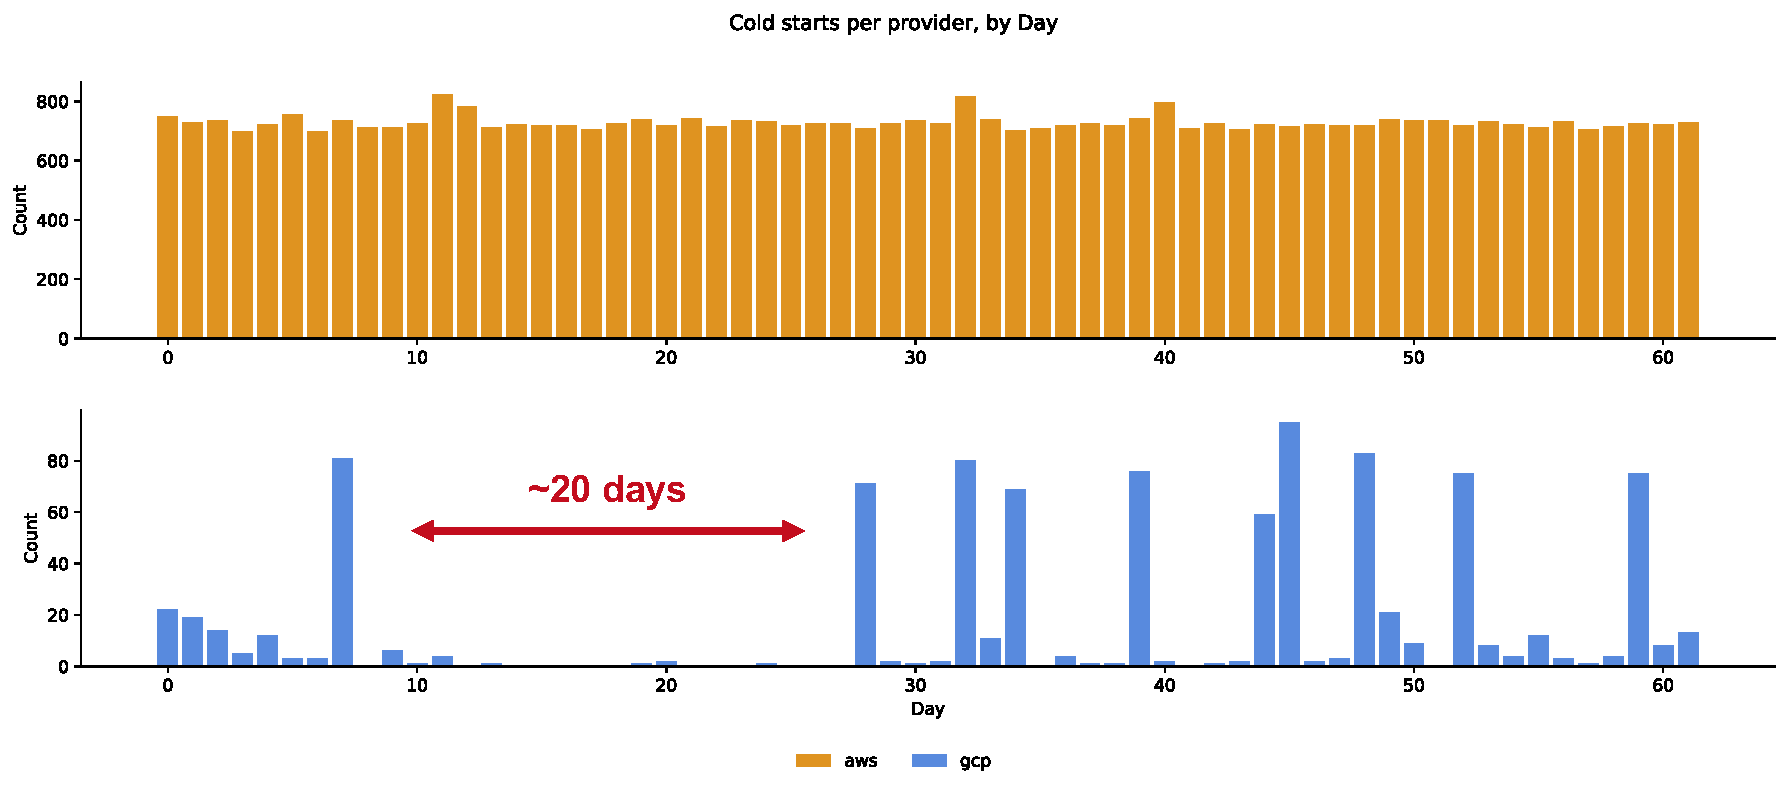
\includegraphics[width=0.95\textwidth]{cold-starts-by-day.pdf}
  \caption{Amount of cold starts per day per provider.}
  \label{fig:cold-starts-per-day-per-provider}
\end{figure}

% ------------------------------------------------------------

% Environment Lifetime and Environment Reuse Metrics

% ------------------------------------------------------------
\subsection{Environment Lifetime and Environment Reuse Metrics}
These two metrics are closely related to the cold start phenomenon. Although not specifically targeted by this benchmark, environment reuse can be beneficial to preserve state between function executions, and potentially reduce amount of work that is required before the handler function can be called. The benchmark used two metrics in this context:
\begin{itemize}
  \item environment lifetime is measured by \emph{durationSinceColdStartMs} metric,
  \item environment reuse is measured by the \emph{handlerCount} metric.
\end{itemize}

\begin{figure}[ht!b]
  \centering
  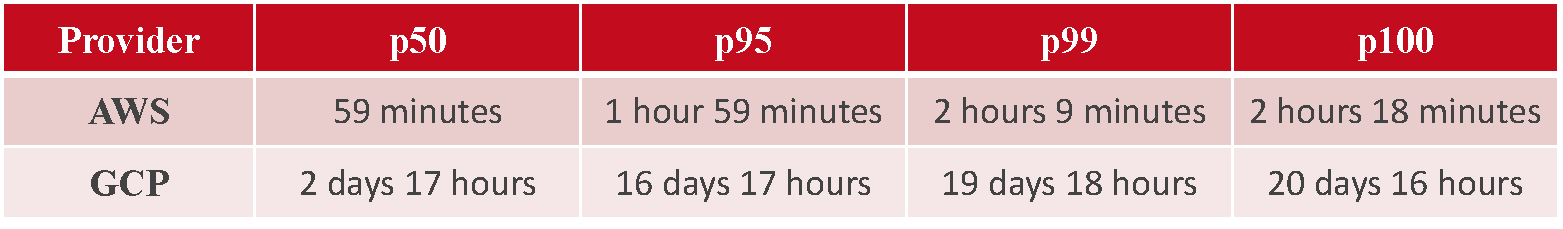
\includegraphics[width=.99\textwidth]{duration-since-cold-start.pdf}
  \caption{\emph{durationSinceColdStart} distribution - environment lifetime per provider.}
  \label{fig:duration-since-cold-start-distributions-per-provider}
\end{figure}

% \begin{figure}[!ht]
%   \centering
%   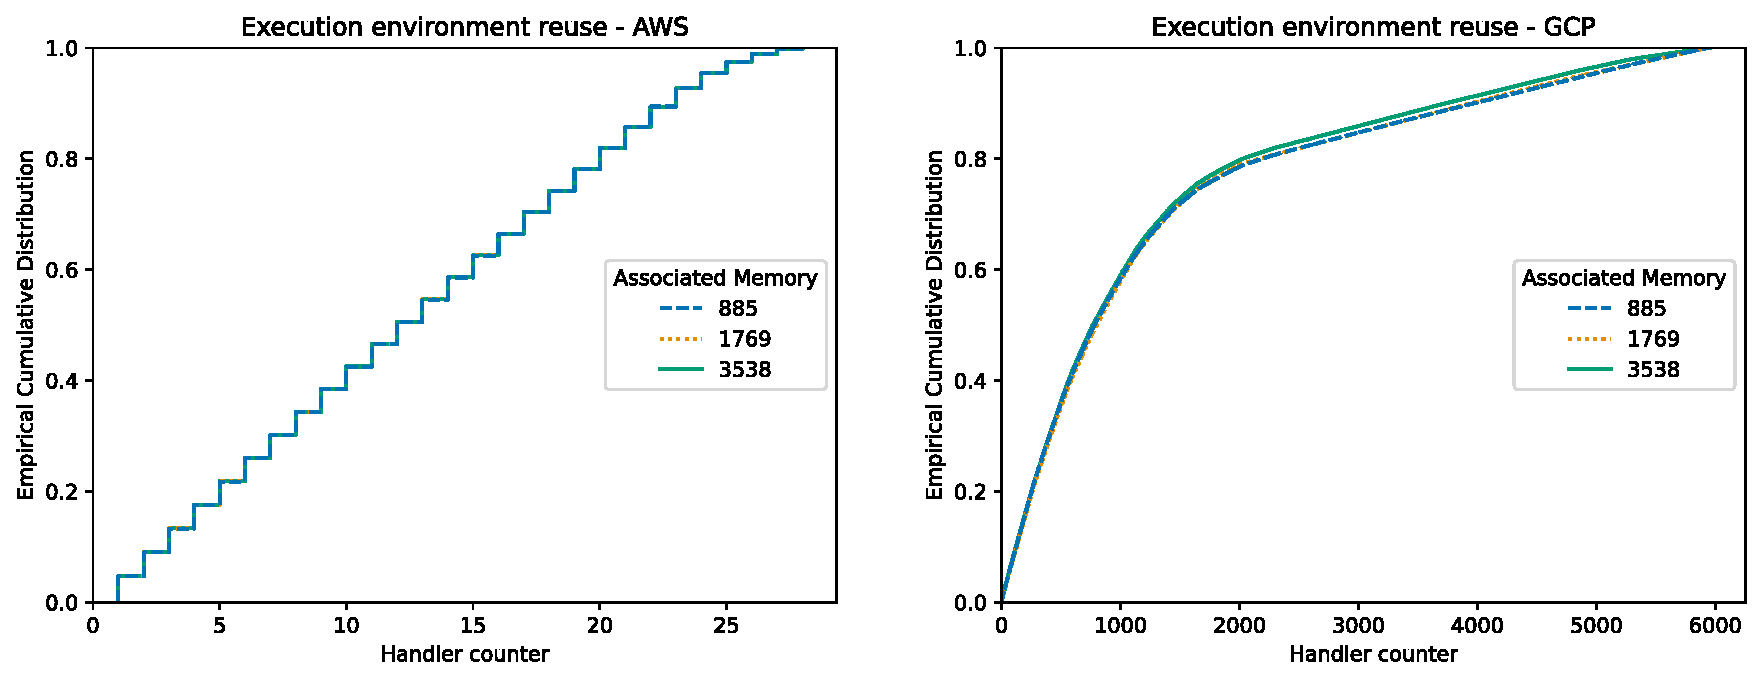
\includegraphics[width=\textwidth]{environment-reuse.pdf}
%   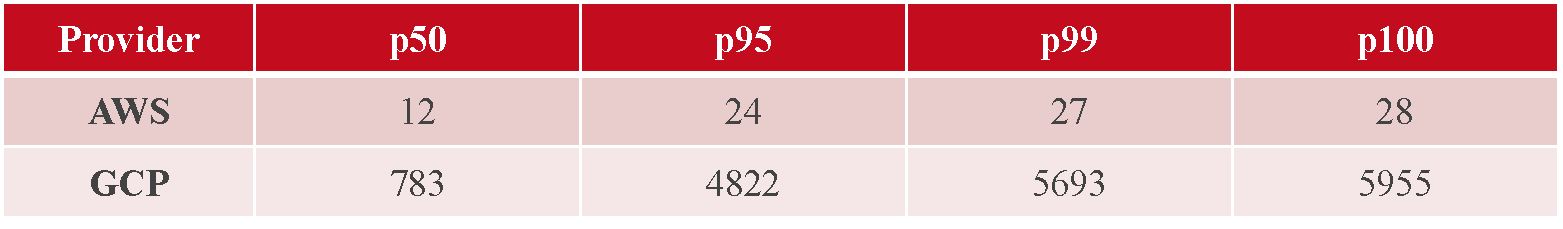
\includegraphics[width=\textwidth]{handler-count.pdf}
%   \caption{\emph{handlerCount} distribution - environment reuse per provider.}
%   \label{fig:env-reuse-per-provider}
% \end{figure}

\begin{figure}[h!t]
  \centering
  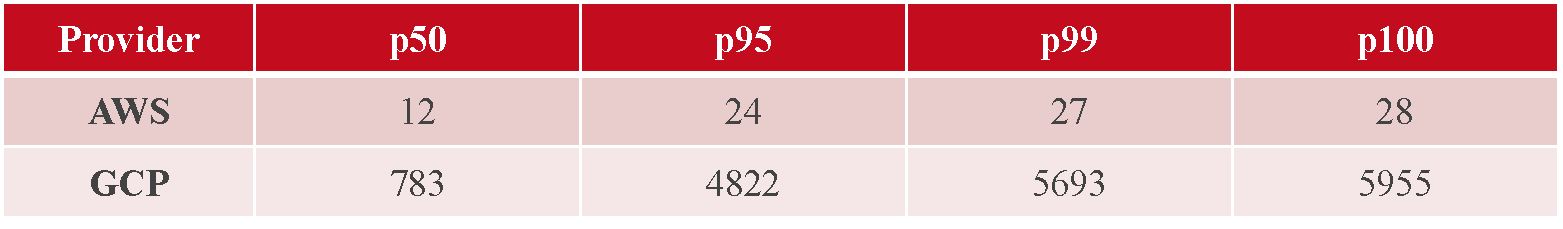
\includegraphics[width=\textwidth]{handler-count.pdf}
  \caption{\emph{handlerCount} distributions per provider.}
  \label{fig:handler-count-distributions-per-provider}
\end{figure}

\begin{figure}[!htb]
  \centering
  
\includegraphics[width=0.75\textwidth]{1-handler-counts-aws.pdf}
  
\includegraphics[width=0.75\textwidth]{1-handler-counts-gcp.pdf}
  \caption{Environment reuse on Lambda (above) and Cloud Run functions (below).}
  \label{fig:env-reuse-per-provider-gcp}
\end{figure}

The longest running Cloud Run function was reusing the environment over 200 times longer than the longest running Lambda function. Environment reuse \textbf{per provider} is consistent across different input images, output formats, output widths and performance settings.

% ------------------------------------------------------------

% IMAGE PROCESSING DURATION

% ------------------------------------------------------------
\subsection{Measuring Image Processing Duration}
This metric determines how quickly optimized images are ready to be delivered to end users. It is measured in millisecond resolution and captures the core operation of transforming images according to specified optimization parameters. It is heavily related to the performance settings, such as amount of compute assigned to the function, output format and width, as well the input image resolution. For completeness, visualization of absolute optimization times is provided for one of the input images in all 54 function variants.

Please note that lower performance settings imply longer processing duration. Different output formats have different computational complexity, with JPEG having the shortest processing times, and AVIF having the longest. Different providers also exhibit difference in processing duration, even for \emph{"the same"} compute (vCPUs) and memory configurations.

\begin{figure}[!htb]
  \centering
  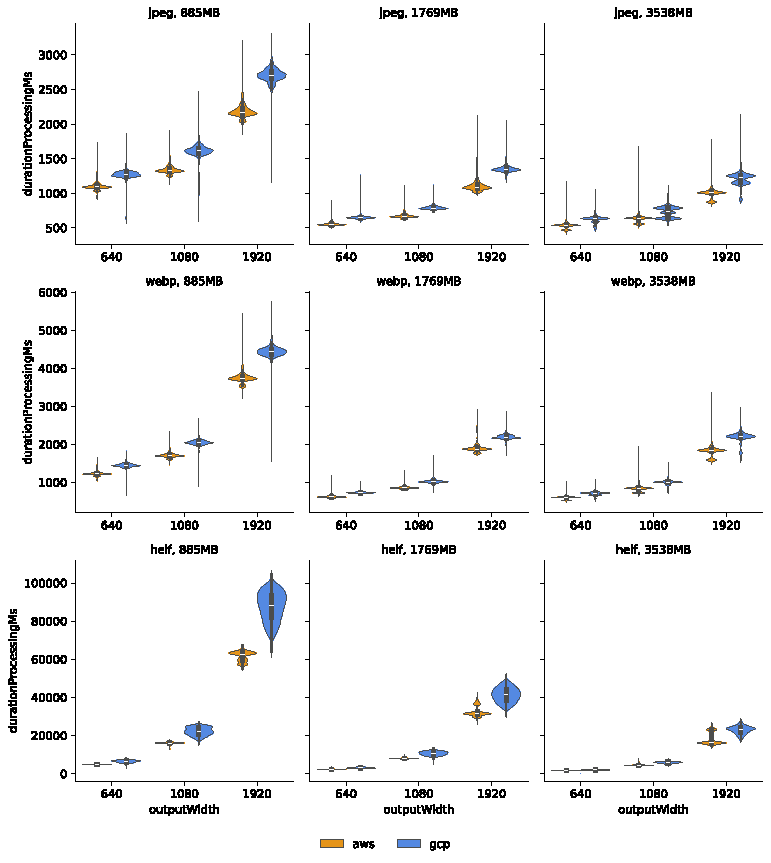
\includegraphics[width=0.99\textwidth]{2-duration-portrait.pdf}
  \caption{Absolute image processing durations \emph{(durationProcessingMs, portrait)}.}
  \label{fig:image-processing-duration-portrait}
\end{figure}


% ------------------------------------------------------------

% TEMPORAL VARIABILITY

% ------------------------------------------------------------
\subsection{Daily Temporal Variability}

The benchmark data shows changes of the processing duration depending on the time of day when the optimization workflow is executed. The variability is the biggest for the AVIF format, and for functions with the most memory assigned for image processing.

\begin{figure}[hb]
  \centering
  
\includegraphics[width=\textwidth]{4-duration-normalized-hod-all.pdf}
  \caption{Average image optimization duration throughout a day in various configurations.}
\end{figure}

In addition to the \emph{hourly} variability, another \emph{minutely} variability is present given the aggregation basis of individual minutes instead of hours. The \emph{hourly variability} is the bigger of the two, around 1\%. The \emph{minutely variability} is lower, usually closer to 0.5\%. This indicates serverless performance changing sharply at the beginning/end of every hour.

\begin{figure}[h!bp]
  \centering
  
\includegraphics[width=\textwidth]{4-duration-normalized-hod.pdf}
  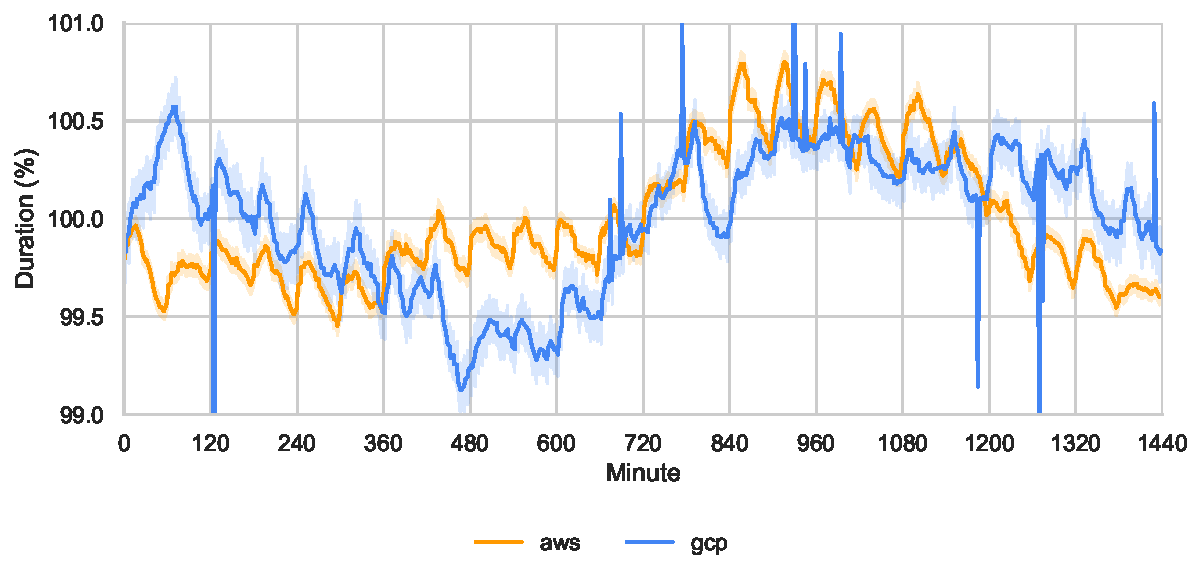
\includegraphics[width=\textwidth]{4-duration-normalized-hod-adjusted-modx.pdf}
  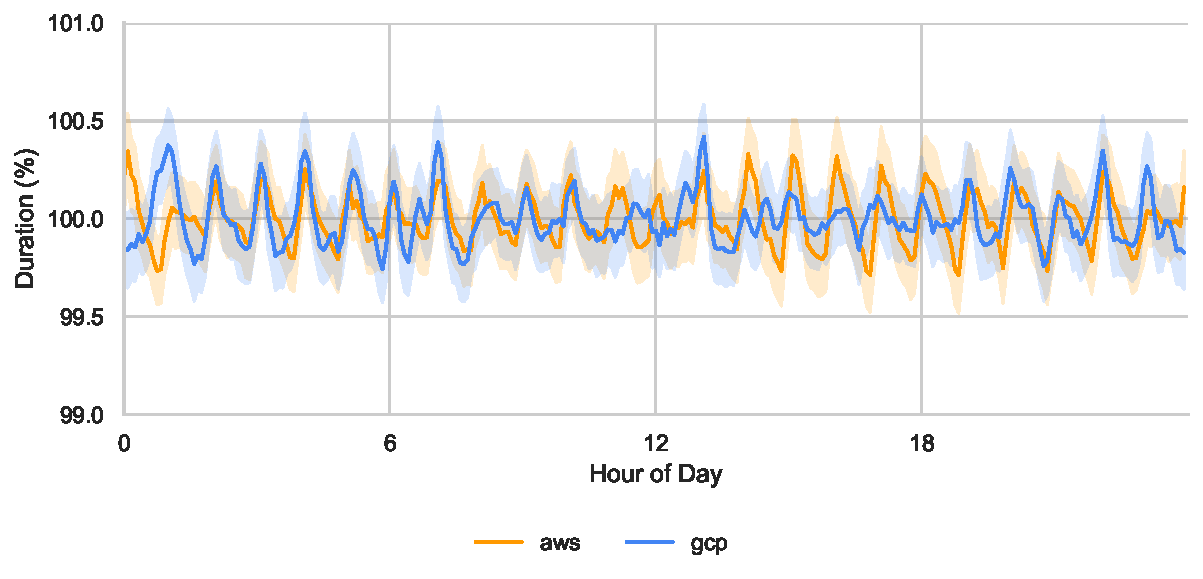
\includegraphics[width=\textwidth]{4-duration-normalized-hod-adjusted.pdf}
  \caption{Average image optimization duration throughout a day in various aggregations.}
\end{figure}



\newpage
\subsection{Weekly Temporal Variability}
The benchmark data also shows changes of the image processing duration depending on the time of week when the optimization workflow is executed. Here, similar to the previous section, we have performed aggregations based on the output format, as well as performance setting assigned to the function. Also, similar to the daily temporal variability, it can be seen that these values are higher for more computationally complex image formats and higher performance settings.

\begin{figure}[hb]
  \centering
  
\includegraphics[width=\textwidth]{4-duration-normalized-how-all.pdf}
  \caption{Average image optimization duration throughout a day in various configurations.}
\end{figure}

\begin{figure}[!htbp]
  \centering
  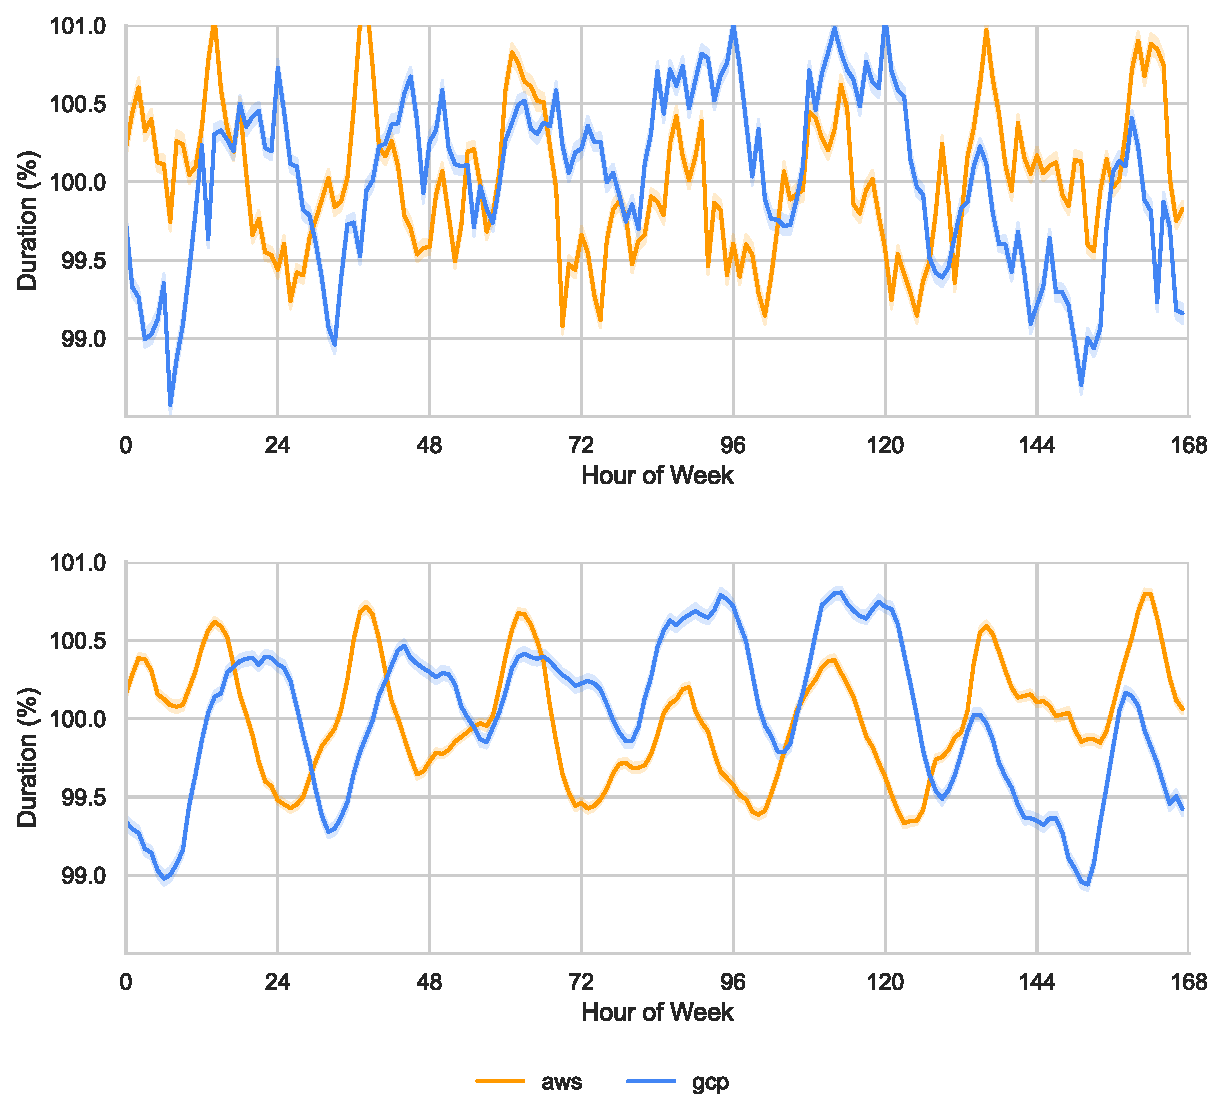
\includegraphics[width=\textwidth]{how.pdf}
\caption{Image optimization duration throughout a week: raw aggregated values (above) and smoothened aggregate based on a rolling average (below).}
\end{figure}






% ------------------------------------------------------------
\newpage
% Environment-related Metrics

% ------------------------------------------------------------
\subsection{Environment-related Metrics}
These metrics exhibited both static and variable behavior over the total duration of the experiment:
\begin{itemize}
  \item \emph{providerArch} - x64 across all function variants on both serverless platforms,
  \item \emph{providerCpus} - variable on AWS, but constant on GCP,
  \item \emph{providerMemoryAvailable} - variable on AWS, but constant on GCP, these metrics represent the actual vCPU and memory available from within the function,
  \item \emph{providerNodeVersion} - v20.18.0 across all function variants.
\end{itemize}

\begin{figure}[!h]
  \centering
  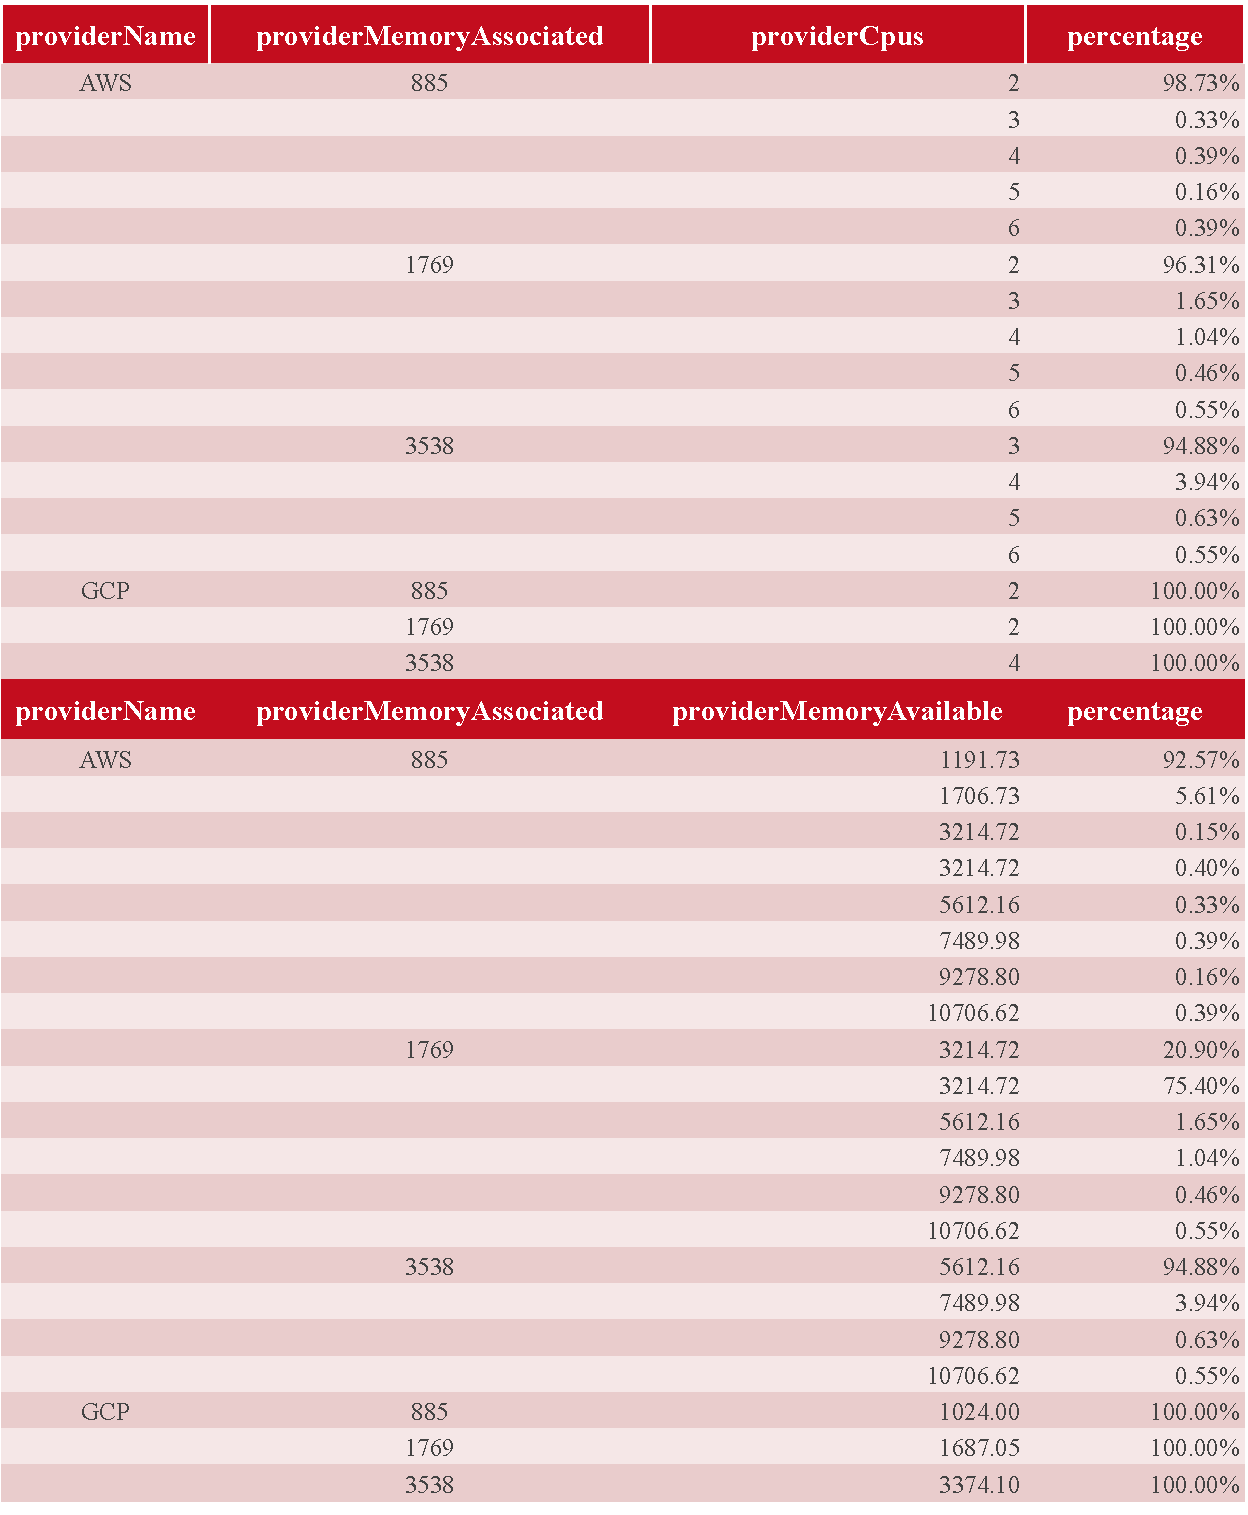
\includegraphics[width=0.9\textwidth]{provider-cpus-memory.pdf}
  \caption{Differences in actual hardware configuration for identical performance setting.}
  \label{fig:provider-cpus-and-memory}
\end{figure}


% ------------------------------------------------------------
\newpage
% Handler Count-Related Duration Variability

% ------------------------------------------------------------
\subsection{Handler Count-Related Duration Variability}
We have observed increased average image processing duration on the first 3 to 6 optimization invocations. This should be not confused with the \emph{cold start latency}. This is the duration of the individual image optimization instruction within the function handler.

On average, the first execution of the image optimization on AWS Lambda is around 7\% higher than baseline. Actually, it is a bit more than that, due to the relative commonness of the cold starts on this platform, and given the p100 handlerCount on AWS Lambda presented in the previous section is only 28. This effect is also noticeable, but not so pronounced on Google Cloud Run functions, where the value reaches only 3\% above the \emph{true} baseline. Please note the difference in the confidence intervals between the providers.

\begin{figure}[!htb]
  \centering
  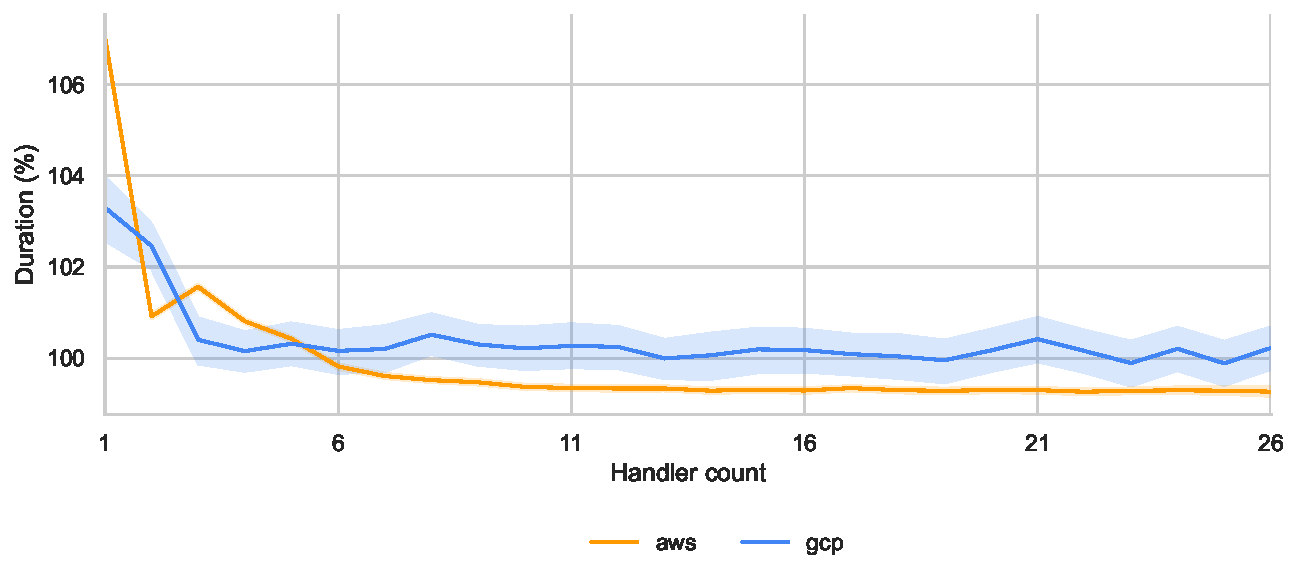
\includegraphics[width=\textwidth]{5-first-25.pdf}
  \caption{Average image processing duration by handler count.}
  \label{fig:image-processing-duration-by-handler-count}
\end{figure}



% ------------------------------------------------------------
\newpage
% Handler Count-Related Duration Variability

% ------------------------------------------------------------






\clearpage
\section{Discussion}
\label{cha:discussion}

% Cold starts were more frequent in lower memory configurations, consistent with the expectation that providers may prioritize keeping higher-resourced environments active. Additionally, we observed that the overall frequency of cold starts decreased as our benchmark progressed, suggesting that the platforms were adapting to the regular invocation patterns established by our scheduled workload generator.

\subsection{Performance variability analysis}
\subsection{User vs operator perspective}
\subsection{Cloud computing as a utility}

% "Three sentences at the end about stuff that didn't work out"

\clearpage
\section{Related Work}
\label{cha:relatedwork}

This chapter explains how this thesis fits within the existing research. We will break down this explanation by looking at research about serverless performance in general and studies focused on image processing in cloud environments.

\subsection{Serverless Performance Research}
Serverless computing is a vibrant area of study, and several benchmarking systems have been created to test Function-as-a-Service (FaaS) platforms.

\cite{kim2019functionbench} presents a collection of tests and real-world examples designed for public cloud services. It includes 4 different categories of benchmarks, including Micro benchmarks, Application benchmarks, ML model training and ML model serving. Image processing is one of the benchmarks in this benchmark suite, however, it is implemented with the Pillow library that we described earlier, that has inferior performance comparing to sharp.

\cite{somu2020panopticon} is another tool for testing serverless applications. It automates the process of setting up tests and running them across different setups and cloud platforms, focusing on stress-testing the application under different configurations. It also supports function chaining. \cite{lloyd2018serverless} describes factors contributing to cold starts, focusing on different states, on the spectrum from cold to warm, of serverless infrastructure. Their research is primarily geared towards container deployments and not directly applicable to ZIP deployments.

\cite{schirmer2023night} looks specifically at performance changes in cloud serverless platforms, especially daily and weekly patterns in how long functions take and when cold starts happen. Their research, which involved frequent benchmarking over two months, revealed significant performance fluctuations throughout the day, with differences of up to 15\%. The study also found an increase in cold starts during peak hours and at the beginning of the week.

\cite{wang2018peeking} studies how well different serverless platforms keep performance separate for different users, which also helps us understand performance changes. They find that AWS Lambda has the best scalability and the lowest cold start latency, followed by Google Cloud Functions (1st gen). However, the lack of performance isolation in AWS between function instances from the same account may cause decrease in IO, networking, or general performance. \cite{dantas2022application} analyzes, we analyze the
performance of the container-based deployment and ZIP-based
deployment of AWS Lambda using a variety of language runtimes
and applications running with different function configurations

\subsection{Image Processing Research}

\clearpage
\section{Conclusion \& Future Work}
\label{cha:conclusion}

This thesis has examined how serverless platforms perform when handling image optimization tasks. Our two-month benchmark comparing AWS Lambda and Google Cloud Run functions across 108 function variants reveals significant differences in how these platforms operate under real-world workloads.

We found that AWS Lambda and Google Cloud Run take fundamentally different approaches to environment management. Lambda recycles execution environments more frequently, which likely improves resource utilization but results in more cold starts. Google Cloud, meanwhile, maintains environments for remarkably long periods - sometimes over 20 days - minimizing cold starts but potentially limiting infrastructure flexibility.

By testing multiple function variants with different performance settings, we discovered that hardware allocation significantly impacts performance variability. More compute-intensive formats like AVIF showed greater sensitivity to underlying infrastructure changes than simpler formats like JPEG, suggesting that as computational demands increase, image optimization becomes more vulnerable to performance fluctuations.

One practical finding is that highly optimized image processing using native libraries works efficiently within serverless ZIP deployments without requiring custom containers. This is good news for developers who want to minimize operational complexity while maintaining processing speed.

Our research adds to the understanding of serverless computing by testing performance through a specific, practical use case. Image optimization makes an excellent test subject for serverless platforms because it's event-driven, has variable computational requirements, and directly impacts user experience in web applications.

We should note that while we tested over 100 variations of image optimizing functions, expanding the parameter space further would create significant logistical challenges. Ideally, a benchmark like ours would test continuous parameter values rather than discrete ones, allowing for more nuanced exploration of the optimization landscape. However, building such a system would require sophisticated frameworks for managing and analyzing high-dimensional data - something beyond our current scope.

Future work could investigate how network latency affects end-to-end image optimization, particularly when retrieving source images from cloud storage. Testing how these functions handle traffic spikes would better simulate real-world conditions. Including more cloud providers would also give a broader view of the serverless ecosystem.

As web performance standards evolve and new image formats emerge, the intersection of serverless computing and image optimization will remain relevant. We hope this research helps developers make informed decisions about serverless image optimization and provides a solid foundation for future performance studies.


% \clearpage
% \section{Appendix}

\newpage
\emergencystretch=0.3pt % fix overfull hboxes in the bibliography
\printbibliography
\end{document}
